%\documentclass[12pt]{report}
%\usepackage{amsmath,graphicx,makeidx}

%\makeindex
%\begin{document}
%\tableofcontents

\chapter{Schematic Creation}
\thispagestyle{empty}
\label{chap5}
The first step in the design of an electronic system is the design of
its circuit. This circuit is usually created using a {\tt Schematic
  Editor}\index{Schematic!editor} and is called a {\tt
  Schematic}. \index{Schematic} eSim uses {\tt Eeschema}
\index{Eeschema} as its schematic editor. Eeschema is the schematic
editor of KiCad.  \index{KiCad} It is a powerful schematic editor
software. It allows the creation and modification of components and
symbol libraries and supports multiple hierarchical layers of printed
circuit design.

\section{Familiarizing the Schematic Editor interface}
\figref{eesch1} shows the schematic editor and the various menu and
toolbars.  We will explain them briefly in this section.
\begin{figure}[h]
\begin{center}
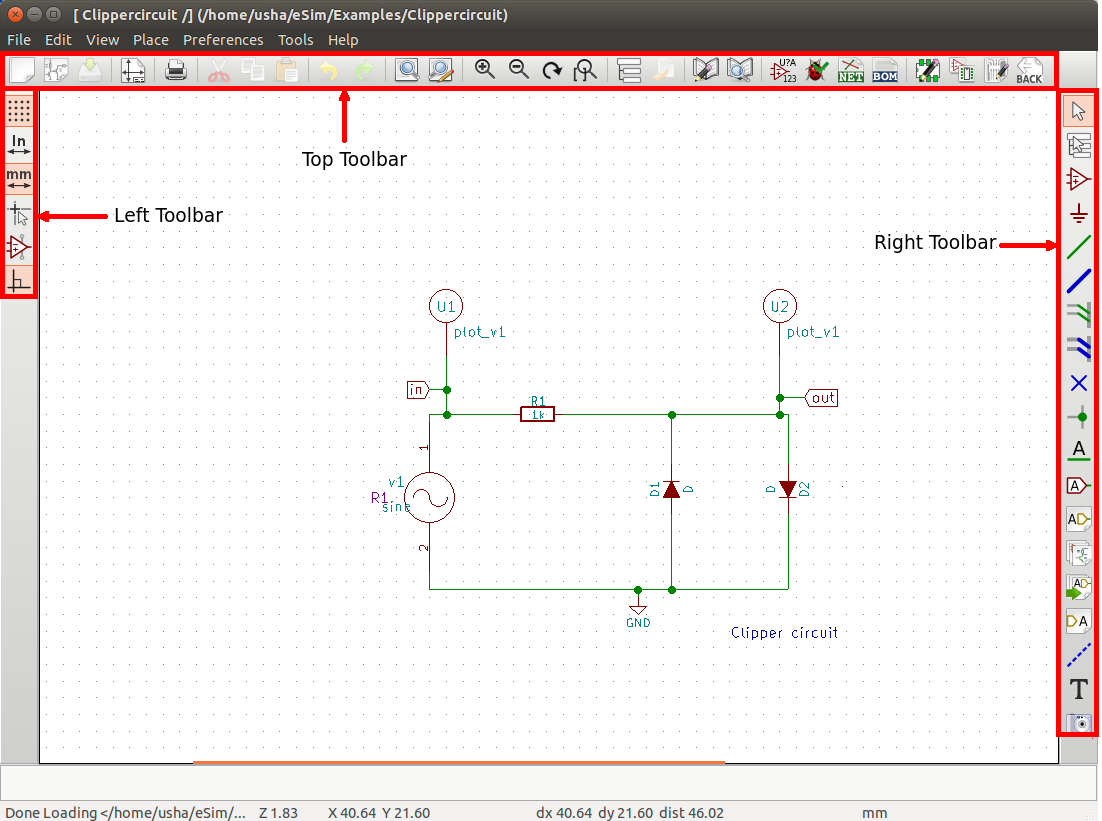
\includegraphics[width=\linewidth]{manual_images/schematic1.png}
%If the fig is appearing too big/small, change the scaling factor 0.2
\caption{Schematic editor with the menu bar and toolbars marked}
\label{eesch1}
\end{center}
\end{figure}

\subsection{Top menu bar}
The top menu bar will be available at the top left corner.
Some of the important menu options in the top menu bar are:

\begin{compactenum}
\item File - 
The file menu items are given below:
\begin{compactenum}
\item New - Clear current schematic and start a new one
\item Open - Open a schematic 
\item Open Recent - A list of recently opened files for loading
\item Save Schematic project - Save current sheet and all its
  hierarchy.
\item Save Current Sheet Only - Save current sheet, but not others in
  a hierarchy.
\item Save Current sheet as - Save current sheet with a new name.
\item Page Settings - Set preferences for printing the page.
\item Print - Access to print menu (See \figref{print}).
\item Plot - Plot the schematic in Postscript, HPGL, SVF or DXF format 
\item Close - Close the schematic editor. 
\end{compactenum}
\begin{figure}[h]
\begin{center}
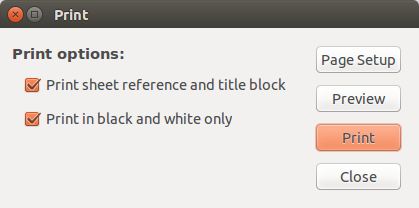
\includegraphics[width=0.5\linewidth]{manual_images/print.png}
\caption{Print options}
\label{print}
\end{center}
\end{figure}

\item Place - 
The place menu has shortcuts for placing various items like
components, wire and junction, on to the schematic editor window. See
\secref{short} to know more about various shortcut keys (hotkeys). 

\item Preferences - 
The preferences menu has the following options:
\begin{compactenum}
\item Component Libraries - Select component libraries and library paths. This enables the user to add the libraries, if the libraries are not loaded in the Eeschema.
\item Schematic Editor Options - Select colors for various items, display 
options and set hot keys.
\item Language - Shows the current list of available languages. Use default. 
\item Import and Export - Contain options to load and save preferences and 
import/ export hot key configuration files. See \secref{short} to know about 
various hotkeys.
\end{compactenum}

\end{compactenum} 

\subsection{Top toolbar}\index{Schematic!toolbar!top}\index{Eeschema!toolbar!top}
Some of the important tools in the top toolbar are discussed
below. They are marked in \figref{eeschem2}.
\begin{figure}[h]
\centering
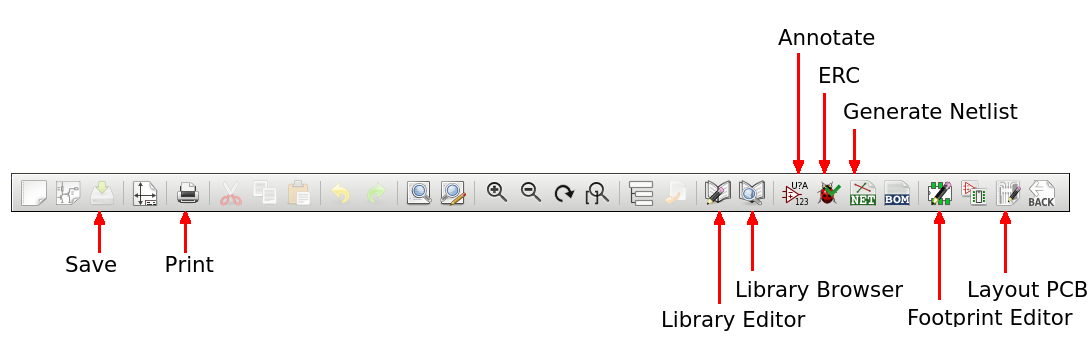
\includegraphics[width=\textwidth]{manual_images/toptoolbar.png}
\caption{Toolbar on top with important tools marked}
\label{eeschem2}
\end{figure}
\begin{compactenum}
\item Save - Save the current schematic
\item Print - Print the schematic
\item Navigate schematic hierarchy - Navigate among the root and
  sub-sheets in the hierarchy
\item Library Editor - Create or edit components.
\item Library Browser - Browse through the various component libraries
  available
\item Annotate - Annotate the schematic
\item Check ERC - Do Electric Rules Check for the schematic
\item Generate Netlist - Generate a netlist for PCB design({\tt .net}) or for
  simulation({\tt .cir}).
\item Create BOM - Create a Bill of Materials of the schematic
\item Footprint editor - Map each component in the PCB netlist to a footprint
\item Layout PCB - Lay tracks between the footprints to get the PCB layout
\end{compactenum}

\subsection{Toolbar on the right}\index{Schematic!toolbar!right}\index{Eeschema!toolbar!right}
The toolbar on the right side of the schematic editor window has many
important tools. Some of them are marked in \figref{eeschem3}.
\begin{figure}[h]
\centering
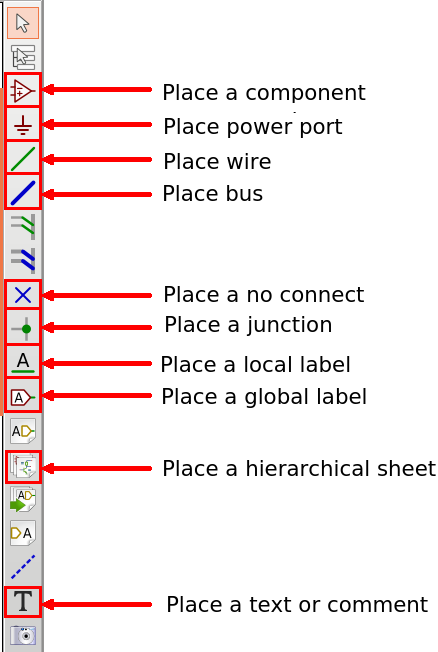
\includegraphics[width=7cm,height=10cm]{manual_images/righttoolbar.png}
\caption{Toolbar on right with important tools marked}
\label{eeschem3}
\end{figure}
Let us now look at each of these tools and their uses.
\begin{compactenum}
\item Place a component - Load a component to the schematic. See
  \secref{selplace} for more details.
\item Place a power port - Load a power port (Vcc, ground) to the schematic.
\item Place wire - Draw wires to connect components in schematic.
\item Place bus - Place a bus on the schematic.
\item Place a no connect - Place a no connect flag, particularly useful in ICs.
\item Place a local label - Place a label or node name which is local to the schematic.
\item Place a global label - Place a global label (these are connected across all schematic diagrams in the hierarchy).
\item Create a hierarchical sheet - Create a sub-sheet within the root sheet in the hierarchy. Hierarchical schematics is a good solution for big projects.
\item Place a text or comment - Place a text or comment in the schematic.
\end{compactenum}
\subsection{Toolbar on the left}\index{Schematic!toolbar!left}\index{Eeschema!toolbar!left}
Some of the important tools in the toolbar on the left are discussed
below. They are marked in \figref{eeschem4}.
\begin{figure}[h]
\centering
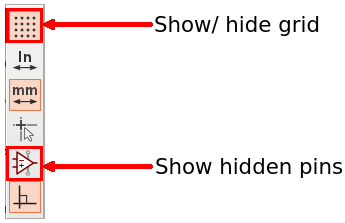
\includegraphics[width=0.4\textwidth]{manual_images/lefttoolbar.png}
\caption{Toolbar on left with important tools marked}
\label{eeschem4}
\end{figure}

\begin{compactenum}
\item Show/Hide grid - Show or Hide the grid in the schematic editor. Pressing the tool again hides (shows) the grid if it was shown (hidden) earlier.
\item Show hidden pins - Show hidden pins of certain components, for  example, power pins of certain ICs. 
\end{compactenum}

\subsection{Hotkeys}
\label{short}
A set of keyboard keys are associated with various operations in the
schematic editor. These keys save time and make it easy to switch from
one operation to another. The list of hotkeys can be viewed by going
to Preferences in the top menu bar. Choose \textit{Schematic Editor Options} and select \textit{Controls} tab. The hotkeys can also be edited here. Some frequently used hotkeys, along with their functions, are given below:
\begin{compactitem}
\item F1 - Zoom in
\item F2 - Zoom out
\item Ctrl + Z - Undo
\item Delete - Delete item
\item M - Move item
\item C - Copy item
\item A - Add/place component 
\item P - Place power component
\item R - Rotate item
\item X - Mirror component about X axis
\item Y - Mirror component about Y axis
\item E - Edit schematic component
\item W - Place wire
\item T - Add text
\item S - Add sheet
\end{compactitem}
\textit{Note: Both lower and upper-case keys will work as hotkeys}. 

\section{eSim component libraries}% \index{Schematic!for
  %simulation} 

eSim schematic editor has a huge collection of components. As Eeschema is  meant  to  be  a  schematic  editor  to  create  circuits  for  PCB,  Eeschema  lacks  some components that are necessary for simulation (e.g.  probes(plot\_v and current sources). A set of component libraries has been created with such components under the label \textit{eSim\_*}. These libraries are Ngspice compatible.  If one is using eSim only  for  designing  a  PCB,  then  one  might  not  need  these  libraries. However, these libraries are essential if one needs to simulate one's circuit. Hereafter, we will refer to these libraries as eSim libraries to distinguish them from libraries already present in Eeschema (Eeschema libraries) as shown in \figref{libraries}.
\begin{figure}[h]
\centering
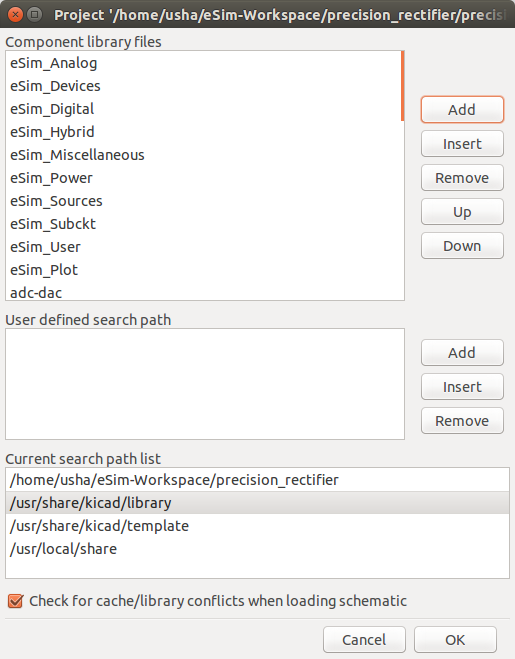
\includegraphics[width=\smfig]{manual_images/libraries.png}
\caption{eSim-Components Libraries}
\label{libraries}
\end{figure}

The following list shows the various eSim component libraries.

\begin{compactitem}
\item \textit {eSim\_Analog} - Contains Ngspice analog models such as aswitch(analog switch), summer(adder model), Transfo(Transformer), zener.
\item \textit {eSim\_Devices} -  Includes elementary components like resistor, capacitor, transistor, MosFet.
\item \textit {eSim\_Digital} -  Includes Ngspice digital models such as basic gates (AND, OR, NOR,NAND,XOR), filpflops (SR, D, JK), buffer, inverter.
\item \textit {eSim\_Hybrid} - Includes components like ADC and DAC.
\item \textit {eSim\_Miscellaneous} -  Contains components like ic(used for giving initial conditions in circuit) and port(used in creating subcircuits).
\item \textit {eSim\_Plot} -  Contains plotting components like plot\_v1 (plot voltage at a node), plot\_v2 (plot voltage between 2 nodes), plot\_i2 (plot current through branch), plot\_log (plot logarithmic voltage at a node).
\item \textit {eSim\_Power} -  Includes power components like DIAC, TRIAC and SCR.
\item \textit {eSim\_Sources} -  Contains sources for the circuits like AC voltage source, DC voltage source, sine source and pulse source.
\item \textit {eSim\_Subckt} -  Contains subcircuit components like Op-Amp(UA 741), IC 555, Half adder and full adder.
\item \textit {eSim\_User} - A repository for all user created components
\end{compactitem}

\section{Schematic creation for simulation} \index{Schematic!for
  simulation} 
There are certain differences between the schematic created for
simulation and that created for PCB design. We need certain components
like plots and current sources for simulation whereas these are not
needed for PCB design. For PCB design, we would require connectors
(e.g. DB15 and 2 pin connector) for taking signals in and out of the
PCB whereas these have no meaning in simulation. This section covers schematic creation for simulation. Refer to \chapref{chap12} to know how to create schematic for PCB design.

The first step in the creation of circuit schematic is the selection
and placement of required components. Let  us  see  this  using  an  example.   Let  us  create  the  circuit schematic of an RC  filter given in \figref{schemfin} and do a transient simulation.  


\subsection{Selection and placement of components}\index{Component!place} 
\label{selplace}
We would need a resistor, a capacitor, a voltage source, ground
terminal and some plot components. To place a resistor on the schematic editor window, select the \textit{Place a component} tool from the toolbar on the right side and click
anywhere on the schematic editor. This opens up the component
selection window. This action can also be performed by pressing
the key A. Choose the \textit{eSim\_Devices} library and click on the arrow near it. This will open the \textit{eSim\_Devices} library and the resistor component can be found here. \figref{resistor} shows the selection of resistor component. Click on {\tt OK}. A resistor will be tied to the cursor. Place the resistor on the
schematic editor by a single click. To place the next component, i.e., capacitor, click again on the schematic editor. The capacitor component is also found under \textit{eSim\_Devices} library. Select it and then click on {\tt OK}. Place the capacitor on the schematic editor by a single click.

\begin{figure}[h]
\centering
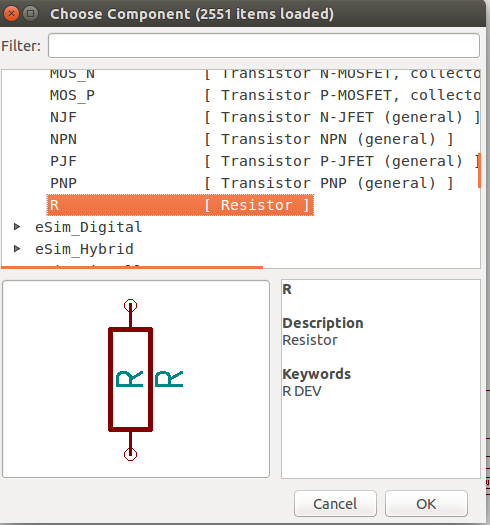
\includegraphics[width=0.5\textwidth]{resistor.png}
\caption{Placing a resistor using the Place a Component tool}
\label{resistor}
\end{figure}
 
Let us now place a sinusoidal voltage source. This is required for performing transient analysis. On the component selection window, choose the library \textit{eSim\_source}. Select the component {\tt SINE} and click on {\tt OK}. Place the sine source on the schematic editor by a single click. Similarly select and place {\tt gnd}, a ground terminal from the {\tt power} library. 

The plot components can be found under the eSim\_Plot library. Select the plot\_v1 component and place the component. Once all the components are placed, the schematic editor would look like as in \figref{afterplace}.
\begin{figure}[h]
\centering
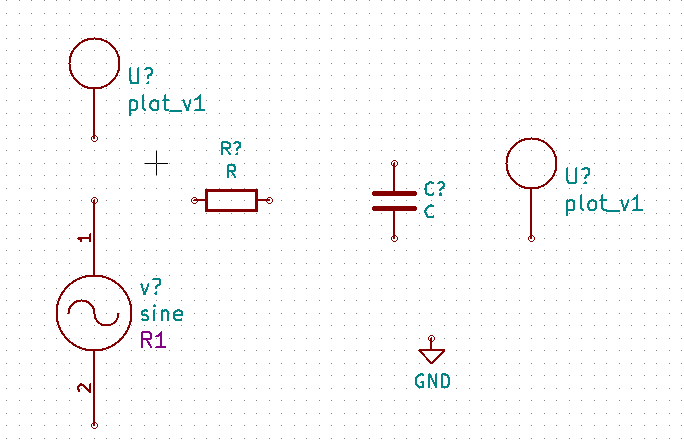
\includegraphics[width=0.63\textwidth]{manual_images/afterplace.png}
\caption{All RC circuit components placed}
\label{afterplace}
\end{figure} 

Let us rotate the resistor to complete the circuit. To rotate the resistor, place the cursor on the resistor as shown in \figref{rotate} and press the key {\tt R}. This applies to all components.\index{Component!rotate}

\begin{figure}[h]
\centering
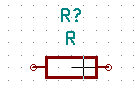
\includegraphics[width=0.3\textwidth]{manual_images/rotate.png}
\caption{Placing the cursor (cross mark) on the resistor component} 
\label{rotate}
\end{figure}

If one wants to move a component, place the cursor on top of the
component and press the key {\tt M}. The component will be tied to the
cursor and can be moved in any direction. \index{Component!move} 

\subsection{Wiring the circuit}
\index{Schematic!wiring}
The next step is to wire the connections. Let us connect the resistor
to the capacitor. To do so, point the cursor to the terminal of
resistor to be connected and press the key {\tt W}. It has now
changed to the wiring mode. Alternately, this can also be done by selecting the \textit{Place wire} tool on the right side toolbar. Move the cursor towards the terminal of
the capacitor and click on it. A wire is formed as shown in
\figref{wire1}. 
\begin{figure}[h]
\centering
\subfloat[Initial stages]{
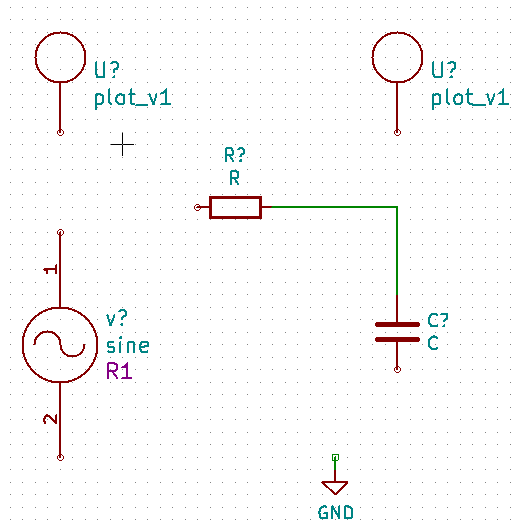
\includegraphics[width=\tnfig]{manual_images/wire1.png}
\label{wire1}} \hfill
\subfloat[Wiring done]{
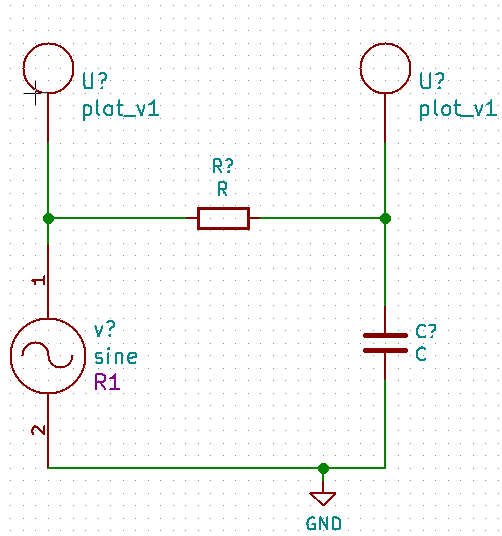
\includegraphics[width=\tnfig]{manual_images/wirefin.png}
\label{wirefin}} \hfill
\subfloat[Final schematic with PWR\_FLAG]{
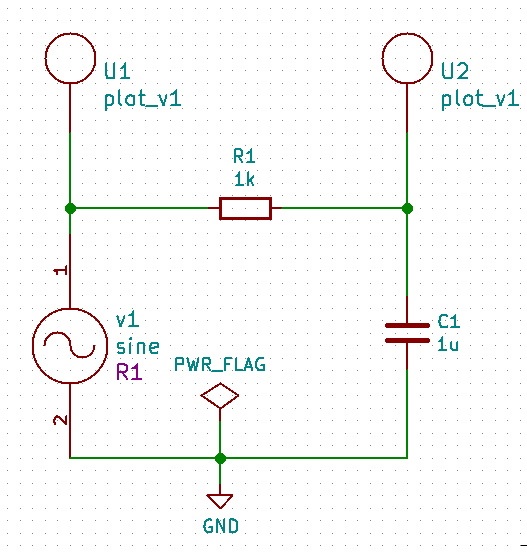
\includegraphics[width=\tnfig]{manual_images/schemfin.png}
\label{schemfin}}
\caption{Various stages of wiring}
\end{figure}
Similarly connect the wires between all terminals and the final
schematic would look like \figref{wirefin}. 

\subsection{Assigning values to components}\index{Component!values}
We need to assign values to the components in our circuit i.e.,
resistor and capacitor. Note that the sine voltage source has been
placed for simulation. The specifications of sine source will be given
during simulation. 
To assign value to the resistor, place the cursor above the letter {\tt R}
(not {\tt R?}) and press the key {\tt E}. Choose \textit{Field
  value}. Type {\tt 1k} in the \textit{Edit value field} box as shown
in \figref{field}. 1k means $1k\Omega$. Similarly give the value
{\tt 1u} for the capacitor. 1u means $1\mu F$.  

\begin{figure}[h]
\centering
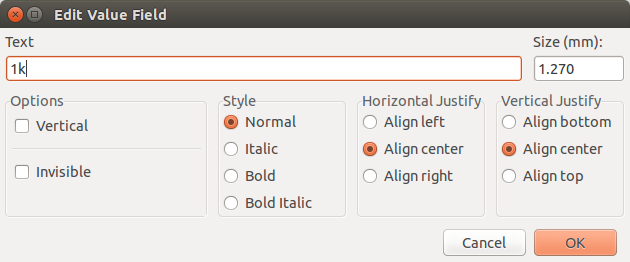
\includegraphics[width=0.5\textwidth]{manual_images/field.png}
\caption{Editing value of resistor}
\label{field}
\end{figure}

\subsection{Annotation and ERC}
\label{ann}\index{Annotate}\index{Schematic!annotate}\index{ERC} \index{Schematic!ERC}
The next step is to annotate the schematic. Annotation gives unique
references to the components. To annotate the schematic, click on
\textit{Annotate Schematic Components} tool from the top toolbar. Click on
{\tt Annotate}, then click on {\tt OK} and finally click on Close as shown in
\figref{anno}. The schematic is now annotated. The question marks
next to component references have been replaced by unique numbers. If
there are more than one instance of a component (say resistor), the
annotation will be done as R1, R2, etc. 

\begin{figure}[h]
\centering
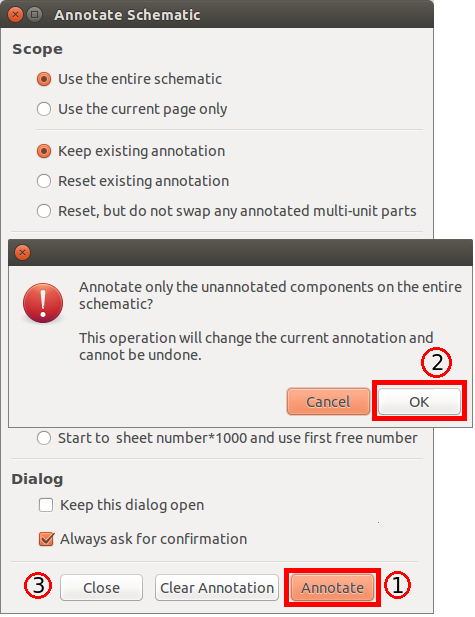
\includegraphics[width=0.45\textwidth]{manual_images/anno.png}
\caption{Steps in annotating a schematic: 1. First click on Annotation then 2. Click on OK then 3. Click on close}
\label{anno}
\end{figure}

Let us now do {\tt ERC} or {\tt Electric Rules Check}. To do so, click
on \textit{Perform electric rules check} tool from the top
toolbar. Click on \textit{Run} button. The error as shown in
\figref{erc} may be displayed. Click on close in the test
erc\index{ERC} window. \index{ERC!error}

\begin{figure}[h]
\centering
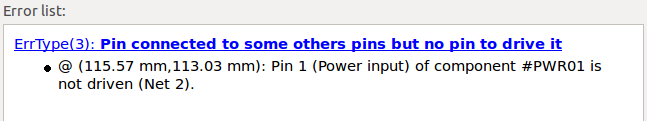
\includegraphics[width=\lgfig]{manual_images/erc2.png}
\caption{ERC error}
\label{erc}
\end{figure}

There will be a green arrow pointing to the source of error in the
schematic. Here it points to the ground terminal. This is shown in
\figref{ercgnd}.

\begin{figure}[h]
\centering
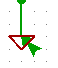
\includegraphics[width=0.1\textwidth]{ercgnd.png}
\caption{Green arrow pointing to Ground terminal indicating an ERC error}
\label{ercgnd}
\end{figure}

This error is due ti the GND pin. The GND pin is a power input pin and Eeschema gives this error as there is no power line connected. To correct this error, a flag has to be placed indicating that there will be an external power line connected to it. Place a {\tt PWR\_FLAG} from the Eeschema 
library \textit{power}. \index{Power Flag} Connect the power flag to the
ground terminal as shown in \figref{schemfin}. %More information about
%PWR\_FLAG is given in \secref{pwr}. One needs to place {\tt PWR\_FLAG}wherever the error shown in \figref{erc} is obtained. 
Repeat the ERC. Now there are no errors. With this we have created the schematic for simulation.

\subsection{Netlist generation}\index{Netlist!for simulation}
\label{chap5-netlist-generation}
To simulate the circuit that has been created in the previous section, we
need to generate its netlist. {\tt Netlist} is a list of components in
the schematic along with their connection information. \index{Netlist}
To do so, click on the \textit{Generate netlist} tool from the top
toolbar. Click on Spice from the window that opens up. Check the
option {\tt Default Format}. Then click on
\textit{Generate}. This is shown in \figref{chap5net}. Save the
netlist. This will be a {\tt .cir} file. Do not change the directory
while saving. 
\begin{figure}[h]
\centering
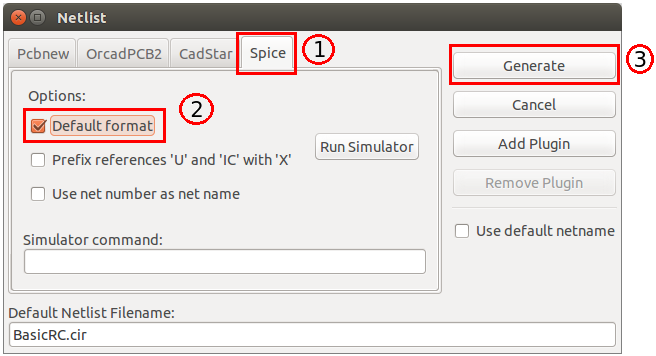
\includegraphics[width=0.6\textwidth]{manual_images/netlist.png}
\caption{Steps in generating a Netlist for simulation: 1. Click on Spice then\\
 2. Check the option {\tt Default Format} then 3. Click on Generate}
\label{chap5net}
\end{figure} 
Now the netlist is ready to be simulated. Refer to \cite{kicad} or \cite{kicad2} to know more about Eeschema.

\section {Tools for creating the PCB layout}
The Eeschema top toolbar also has two important tools which can help the user to generate the PCB layout of the created schematic.

\subsection {FootPrint Editor}
Clicking on the \textit{Footprint Editor} tool will open the {\tt CvPcb} 
\index{CvPcb} window. This window will ideally open the .net file for the 
current project. So, before using this tool, one should have the netlist 
for PCB design (a .net file). To know more about how to assign footprints 
to components, see \chapref{chap12}.

\subsection {PCB Layout}
Clicking on the \textit{Layout Editor} tool will open {\tt
Pcbnew}\index{Pcbnew}, the layout editor used in eSim. In this
window, one will create the PCB. It involves laying tracks and vias,
performing optimum routing of tracks, creating one or more copper
layers for PCB, etc. It will be saved as a {\tt .brd} file in the 
current project directory. \chapref{chap12} explains how to use the 
\textit{Layout Editor} to design a PCB. 


%\printindex
%\end{document}
